\documentclass[parskip=full]{scrartcl}
\usepackage[T1]{fontenc}    % avoid garbled Unicode text in pdf
\usepackage[utf8]{inputenc} % use utf8 file encoding for TeX sources
\usepackage[german]{babel}  % german hyphenation, quotes, etc
\usepackage{hyperref}       % detailed hyperlink/pdf configuration
\hypersetup{                % ‘texdoc hyperref‘ for options
pdftitle={PSE: Entwicklung eines relationalen Debuggers - Implementierungsdokument},%
,%
}
\usepackage{graphicx}       % provides commands for including figures
\usepackage{csquotes}       % provides \enquote{} macro for "quotes"
\usepackage[nonumberlist]{glossaries}     % provides glossary commands
\usepackage{enumitem}
\usepackage{xcolor}
\usepackage{verbatimbox}
\usepackage{lscape}
\newcommand\frage[1]{\textcolor{red}{#1}}


\font\myfont=cmr12 at 16pt

\title{
	\vspace{2cm}
	\myfont 
	Praxis der Softwareentwicklung:\\ 
	Entwicklung eines relationalen Debuggers\\
}
\subtitle{
	\vspace{1cm}
	\myfont
	Implementierungsdokument
}
\author{
	\vspace{1cm} \\
	Benedikt Wagner\\
	\texttt{udpto@student.kit.edu}
	\and \vspace{1cm} \\ Chiara Staudenmaier\\
	\texttt{uzhtd@student.kit.edu}
	\and Etienne Brunner\\
	\texttt{urmlp@student.kit.edu}
	\and Joana Plewnia\\
	\texttt{uhfpm@student.kit.edu} 
	\and Pascal Zwick\\
	\texttt{uyqpk@student.kit.edu}
	\and Ulla Scheler\\
	\texttt{ujuhe@student.kit.edu}
	\vspace{1cm}
	\and Betreuer: Mihai Herda, Michael Kirsten
	\vspace{4cm}
}


\begin{document}
\clearpage
\maketitle
\pagenumbering{gobble}
\newpage

\tableofcontents
\newpage
\pagenumbering{arabic}

\section{Einleitung}
Dieses Dokument beschreibt die Ergebnisse der Implementierungsphase (\textit{08.01.-02.02.2018}) im Rahmen des Moduls Praxis der Softwareentwicklung (PSE) am Lehrstuhl \enquote{Anwendungsorientierte formale Verifikation - Prof. Dr. Beckert} am Karlsruher Institut für Technologie (KIT).\\
Hierbei handelt es sich um die Implementierung des Produkts \textit{DIbugger}, welches im Pflichtenheft definiert und während der Entwurfsphase entworfen wurde.

Das eigentliche Produkt dieser Phase ist über folgendes GitHub-Repository verfügbar: \href{https://github.com/JoanaP1997/PSE/tree/dev/Iplementierung}{https://github.com/JoanaP1997/PSE/tree/dev/Iplementierung} \\
Die abgegebene Version wurde mit \textit{prerelease\_v0.1} getaggt.

\begin{figure}[!h]
\centering

\includegraphics[width=0.8\textwidth]{../Plichtenheft/logo_nongi.png}
\caption{Produktlogo}
\end{figure}

\section{Zeitablauf}
Um eine reibungslose Implementierung zu ermöglichen, muss ein gut durchdachter Zeitablauf existieren.
Dieser wurde folgendermaßen umgesetzt:\\
Begonnen wurde mit dem \textit{FileHandler} und dem \textit{UserInterface}. Diese konnten unabhängig voneinander implementiert werden.
Aus Zeitgründen verschob sich der Start der \textit{Control} Implementierung um wenige Tage.
Die Unterpakete der \textit{DebugLogic} wurden in planmäßiger Reihenfolge begonnen. Dabei wurde die \textit{DebugControl} nun parallel zum \textit{Interpreter} entwickelt.
Weiter gab es hier eine Änderung der Verantwortlichkeit. Hierbei implementierte nun Ulla mit an dem Interpreterpaket, wobei Pascal nun den Debugger übernahm.
%folgend ein Bescheuerter Satz
Aus Interessen- und Vorwissensgründen wurde dies so abgesprochen und umgesetzt.
%Aufgrund des Vergessens von simplen Getter / Setter Methoden während des Entwurfs des Pakets \textit{FileHandler.Facade} hat sich die angedachte Entwicklungszeit stark vergrößert, da immer wieder kleine Änderungen vorgenommen werden mussten.%
Der aufwändigste Teil der Implementierung war, wie auch im Entwurf erarbeitet, der \textit{Interpreter}. Insgesamt gestaltete sich aber auch die Implementierung der Benutzeroberfläche des Paketes \textit{UserInterface} zeitintensiver als erwartet.
Das folgende Gantt-Diagramm zeigt den Zeitverlauf in graphischer Form auf.
\begin{figure}[!h]
\centering
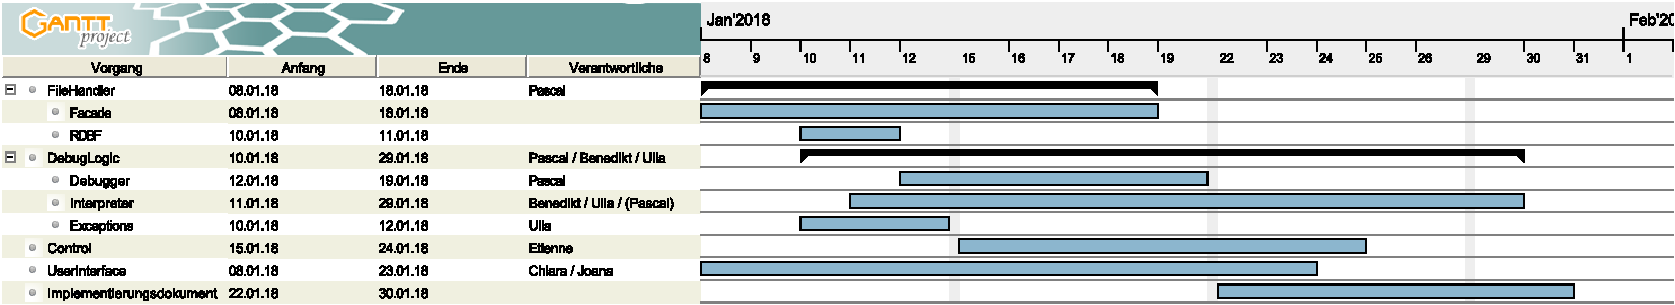
\includegraphics[width=1.0\textwidth]{ganntDiagramm_neu_crop.pdf}
\caption{Gantt-Diagramm des Zeitverlaufes}
\end{figure}

\section{Umsetzung der nichtfunktionalen-Anforderungen}

Die Einteilung der nichtfunktionalen Anforderungen in Unterkapitel orientiert sich an der Anordnung im Pflichtenheft.

	\subsection{Produktdaten}
	Konfigurations-, Sprach- und Einstellungsdateien erfüllen die Funktionalität, die im Pflichtenheft unter 4.2.1 definiert wurde.
%		\begin{itemize}
%		
%		
%			\item[/PD10/] Konfigurationsdateien: \\
%			Diese Dateien speichern eine Konfiguration des Produkts. 
%			Hierzu gehört der aktuelle Status der Benutzeroberfläche (Eingabewerte, Schrittgrößen, Variablenauswahl, Programmtexte, Breakpoints, bedingte Breakpoints, Watch-Expressions) und der Programme.
%			Hier werden dann zusätzlich die aktuellen Positionen in den Programmabläufen gespeichert.
%			
%			\item[/PD20/] Sprachdateien: \\
%			Diese Datei speichert die Übersetzung der gesamten Benutzeroberfläche.
%			Dazu gehören die Texte der GUI-Elemente und Tooltips.
%			
%			\item[/PD30/] Einstellungsdatei: \\
%			Diese Datei speichert die zuletzt ausgewählte Sprache und die Adresse der Konfigurationsdatei, welche zur zuletzt verwendeten Konfiguration passt.  
%			\end{itemize}
			
			 
		\subsection{Produktleistungen}
		%Zeitverhalten, Genauigkeit, Fehlertoleranz
		\begin{itemize}
		\item[/PL10/] Zeitverhalten: \\ NN
%		Das Produkt ermöglicht das Hinzufügen von Eingabevariablen, Watch-Expressions, Schrittgröße und Breakpoints ohne spürbare Verzögerung. Das Ausführen von Schritten, Step-Over und Step-Out, sowie das Erreichen des nächsten Breakpoints, ist ebenfalls ohne spürbare Verzögerung möglich. \\
		%Den Debugmodus zu starten dauert unter 5 Sekunden. 

		\item[/PL20/] Genauigkeit: \\
		Da die Sprache alle primitiven Datentypen von Java unterstützt und diese im Produkt durch äquivalente Java Typen, laufend auf einer JVM (Java Virtual Machine), implementiert wurden, ergeben sich dieselben Genauigkeiten auch in WLang. 

		\item[/PL30/] Fehlertoleranz: \\ NN
%		Durch automatische Warnung bei kritischen Eingaben (A10, A20) und Überprüfung der Semantik, ergibt sich eine hohe Fehlertoleranz bezüglich Benutzereingaben.
%		Durch die automatische Generierung von fehlenden Benutzerangaben für Eingabewerte (FA215), wird der Start des Debugmodus aus dem Editiermodus bei korrektem Programmtext zu jeder Zeit ermöglicht.
%		Über andere Arten von Fehlern wird der Benutzer mittels Pop-Ups informiert.
		\end{itemize}
		
		Unter dem Punkt \enquote{Qualitätsanforderungen an das System} wurde im Pflichtenheft außerdem genannt:
		\begin{itemize}
		\item Richtigkeit: \\
		Die Richtigkeit wurde im Pflichtenheft als sehr relevant eingestuft. Die Implementierung hat dies so weit wie möglich berücksichtigt. Die tatsächliche Umsetzung kann allerdings erst während der Qualitätssicherung sichergestellt werden.
		\end{itemize}
		
		\subsection{Weitere nichtfunktionale Anforderungen}
		%Benutzbarkeit, Wartbarkeit, Erweiterbarkeit, Gesetze/Normen/Sicherheit/Urheberrecht, Robustheit
		\begin{itemize}
		\item[/NA10/]Erweiterbarkeit: \\
		Die Erweiterbarkeit wurde durch klare Pakettrennung, Fassadenklassen als Eintrittstellen in die Pakete und die Definition von Interfaces und abstrakten Klassen (z.B. die abstrakte Klasse \textit{InputValueSuggestion} im Paket \textit{debuglogic.debugger}) sichergestellt und erleichtert.
		\item[/NA20/]Wartbarkeit: \\
		Zunächst fördert die eben dargelegte Umsetzung der Erweiterbarkeit natürlich auch die Wartbarkeit des Produktes. Während der Implementierung wurde außerdem auf eine vollständige und verständliche Dokumentierung Wert gelegt. Die Einarbeitungszeit in den Programmcode wird so verringert.
		\item[/NA30/]Urheberrecht: \\
		Die geplante Open Source Lizenz \href{https://www.gnu.org/licenses/gpl-3.0.de.html}{GNU GPL 3 (GNU General Public License)} wurde im GitHub-Repository als Lizenz eingetragen.
		
		\item[/NA40/] Sicherheit: \\
		Da das Produkt keine Netzwerkverbindung nutzt, verbleiben die vom Benutzer eingegebenen Daten zumindest im Zuständigkeitsbereichs des Programmes ausschließlich auf dem Rechner des Benutzers.
		\item[/NA50/]Benutzerfreundlichkeit: \\ NN
%		Durch das Hilfemenü werden dem Benutzer die wichtigsten Funktionen und deren Anwendung des Produkts erklärt. Erklärungen zu Bestandteilen der Benutzeroberfläche sind durch Tooltips abgedeckt. \\
%		Durch die strikte Trennung der verschiedenen und Gruppierung der zusammengehörigen Elemente der Benutzeroberfläche ergibt sich ein übersichtliches Erscheinungsbild. 
		\end{itemize}
		
				Unter dem Punkt \enquote{Qualitätsanforderungen an die Benutzeroberfläche} wurden im Pflichtenheft außerdem genannt:
				\begin{itemize}
				\item Verständlichkeit \\
				NN
				\item Übersichtlichkeit \\
				NN
				\item Erlernbarkeit \\
				NN
				\item Modifizierbarkeit \\
				NN
				
				\end{itemize}
		
\section{Umsetzung von Entwurfsentscheidungen}
%\subsection{Model-View-Control}
%\subsection{Das Observerpattern}
%z.B. Gui-Facade
%\newpage
\subsection{Singleton}
%%z.B. Command Panel
Durch die Nutzung von Rekursion und des Singletons der Klasse RDBFParser, siehe Abbildung \ref{loadRDBF}, kann das Einlesen einer RDBF (Relational DIbugger File) Datei in einer kurzen Methoden geschehen.
Über \textit{evaluateLineType(String line)} wird der Typ einer Zeile herausgefunden. Je nachdem, von welchem Typ diese Zeile dann ist, werden über das Singleton der Klasse RDBFParser unterschiedliche Methoden aufgerufen, um eine Zuweisung oder einen Block zu erstellen und in der Dateistruktur einzuordnen. Dies ist durch das Singleton einfach zu lösen.
\begin{figure}[!h]
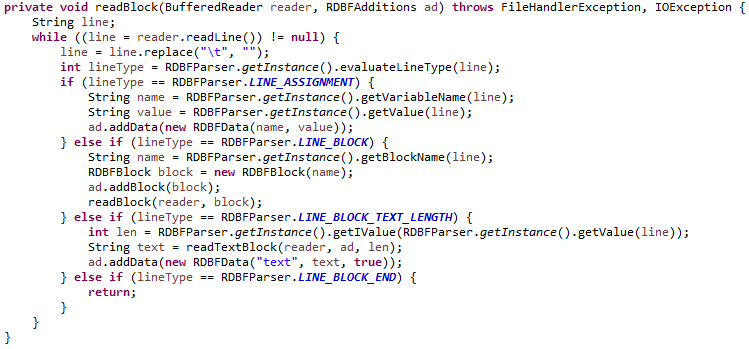
\includegraphics[width=1.0\textwidth]{document_data/loadRDBFFile.png}
\caption{Nutzung des Singletons der Klasse RDBFParser}
\label{loadRDBF}
\end{figure}

%\subsection{Fassade}
%z.B. Control-Facade

\newpage
\subsection{Strategie}
%z.B. FileWriter
\begin{figure}[!h]
\centering
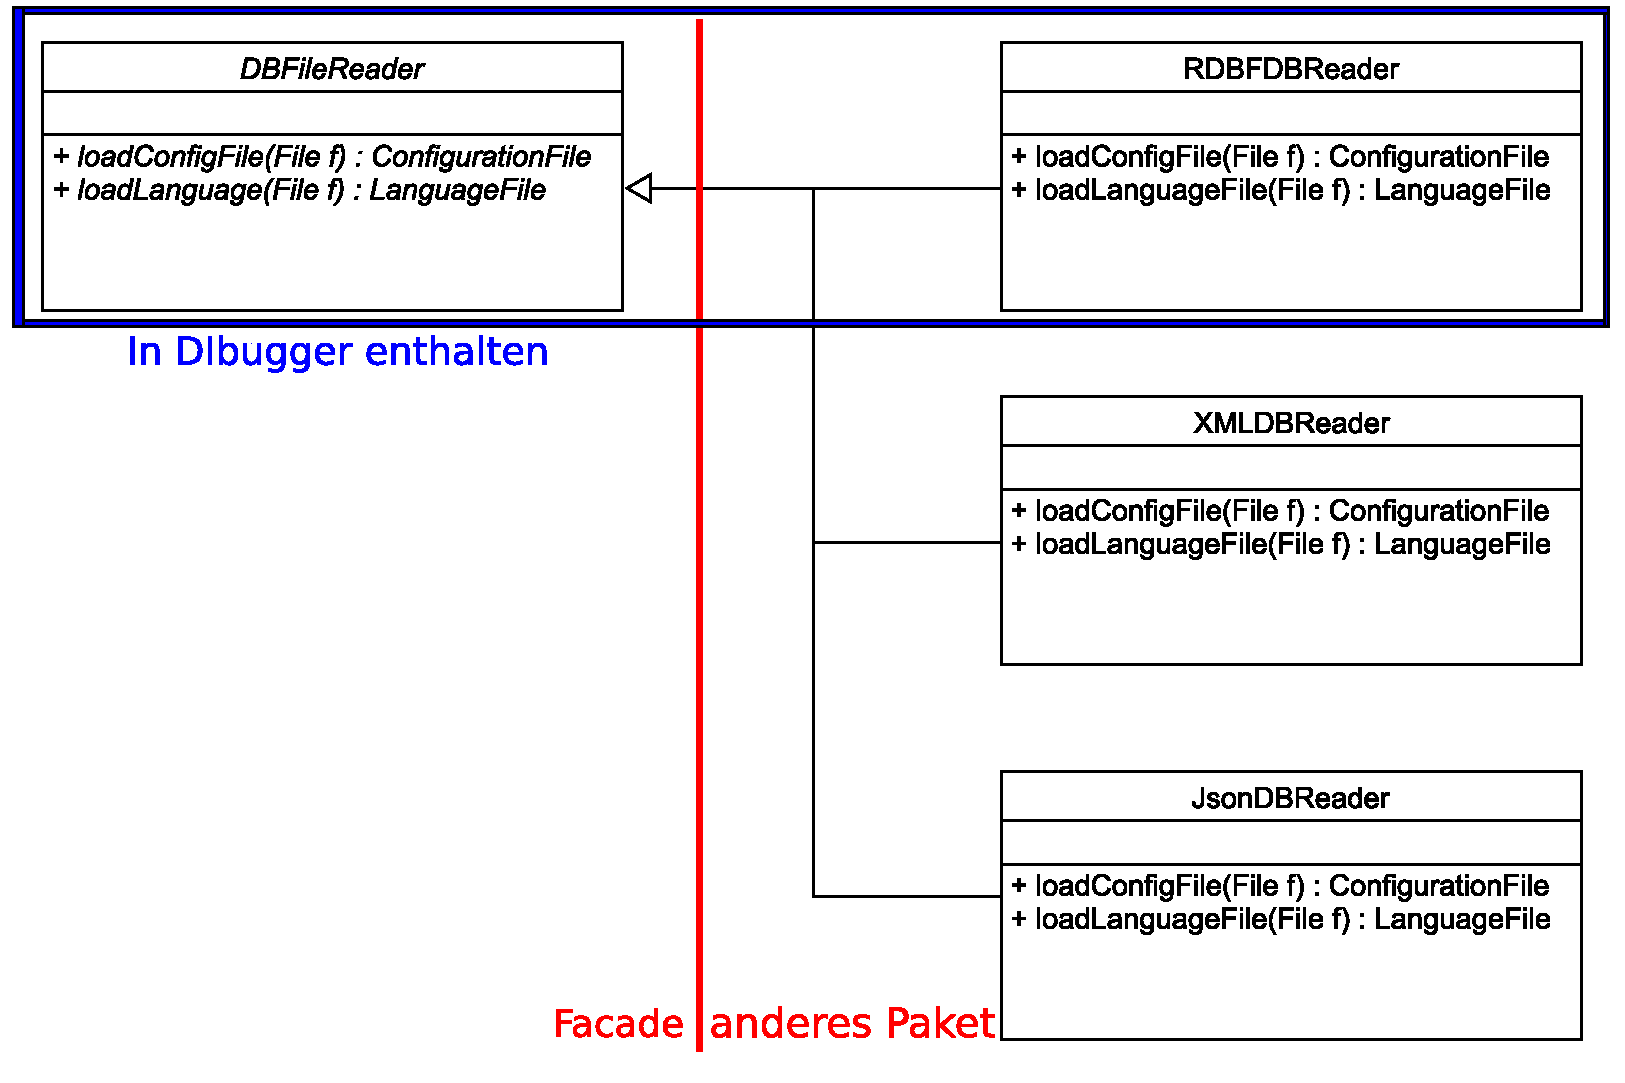
\includegraphics[width=0.8\textwidth]{document_data/Strategy_uml_d.pdf}
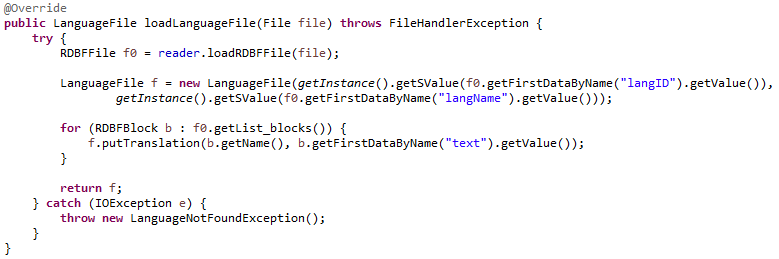
\includegraphics[width=1.0\textwidth]{document_data/loadLangFile.png}
\caption{Strategiemuster des DBFileReaders im Paket FileHandler}
\label{fig:strategy_fh}
\end{figure}
Wie in Abbildung \ref{fig:strategy_fh} aufgezeigt, steht der DBFileReader für den \enquote{Kopf} des Strategiemusters.
Dieser kann als abstrakte Klasse nicht erzeugt werden und stellt zwei abstrakte Methoden ohne Implementierung zur Verfügung.
Diese müssen bei der Vererbung durch eine Unterklasse, z.B. \textit{RDBFDBFileReader}, \textit{XMLDBFileReader}, \textit{JsonDBFileReader} usw., überschrieben und vollständig Implementiert werden.
Dadurch können unter Vorraussetzung einer korrekten Implementierung der beiden Methoden weitere Dateiformate hinzugefügt werden.
Dies gilt ebenso für die Klassen \textit{DBFileWriter, PropertiesFileReader} und \textit{PropertiesFileWriter}. Sie sind ähnlich aufgebaut zu der hier gezeigten Klasse.

\subsection{Die Visitor im Interpreter} Der Entwurf sah im Paket \textit{Interpreter} zwei Klassen vor, die das Visitor Pattern umsetzen. Die beiden Klassen \textit{CommandGenerationVisitor} und \textit{TermGenerationVisitor} sind Unterklassen der von Antlr generierten Klasse \textit{WlangBaseVisitor<T>}, wobei der Generic hier angibt, welchen Datentyp die visit-Methoden zurückgeben. Wie es der Name andeutet, ist dies zum einen die Klasse \textit{Command} und zum anderen die Klasse \textit{Term}. 
Da Terme sowohl während der Traceerzeugung (genauere Erklärung dazu ist im Entwurfsdokument Kapitel 8.10 zu finden) als auch innerhalb von Watch-Expressions und bedingten Breakpoints vorkommen, kam das Problem auf, dass der \textit{TermGenerationVisitor} zunächst sowohl vom \textit{TermsBaseVisitor} (für die im Entwurfsdokument Anhang 12.2 definierte Syntax der Watch-Expressions) als auch vom \textit{WlangBaseVisitor} (für die in Entwurfsdokument 12.1 definierte Wlang-Syntax) erben musste. In Java ist bekanntlich keine Mehrfachvererbung möglich. Zur Lösung des Problems wurden die Grammatiken zusammengefügt und entsprechend beim Verwenden eine andere Startregel angegeben. 
\subsection{Nutzung der von Antlr generierten Klassen}
In Abbildung \ref{createTerm} ist die Nutzung der von Antlr generierten Klassen im Rahmen einer Watch-Expression zu sehen. Diese ist sehr kompfortabel und weicht bei der Nutzung für die Tracegenerierung lediglich in Zeilen 70-72 ab. Hier wird dann eine andere Startregel ausgewählt und der \textit{CommandGenerationVisitor} genutzt. Im abgebildeten Code ist vorher in \texttt{this.specifier} der String gespeichert worden, der die Watch-Expression spezifiziert. Die Klassen \textit{WlangLexer} und \textit{WlangParser} erzeugen dann einen Ableitungsbaum, den \textit{ParseTree}. Über diesen werden die oben angesprochenen Visitor geschickt.
\begin{figure}[!h]
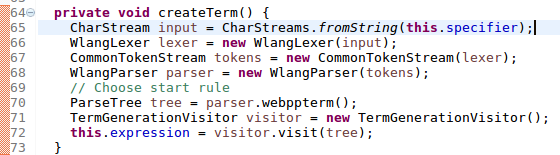
\includegraphics[width=0.7\textwidth]{document_data/createTerm.png}
\caption{Aufrufen der von Antlr erzeugten Klassen}
\label{createTerm}
\end{figure}

\subsection{Umsetzung der Commands}
Die Klassen \textit{Command} und ihre Unterklassen wurden wie im Entwurfsdokument spezifiziert als Kompositum implementiert. Dabei haben zusammengesetzte Subklassen wie der \textit{WhileCommand} immer eine \textit{addChild(Command child)}-Methode. Spannend an den Commands ist vor allem die Umsetzung ihrer \textit{run()}-Methode. Diese ist einer der wichtigsten Teile der Umsetzung des Interpreterpaketes. Sobald sich hier ein Fehler einschleicht, werden die Programmausführungen fehlerhaft. Deshalb wird es wichtig sein, in der Qualitätssicherungsphase diesen Teil besonders ausgiebig zu testen. Bereits in der Implementierung wurden die Commands durch Unittests auf ihr Verhalten überprüft. 
Als einfaches Beispiel betrachten wir in Abbildung \ref{runWhile} die \textit{run()}-Methode der Klasse \textit{WhileCommand}. Hier wird der Nutzen des Kompositum Musters ersichtlich.
Zunächst wird in jedem Command der aktuelle \textit{Scope} vom hauptverantwortlichen \textit{GenerationController} \texttt{this.controller} geholt. In einfachen Befehlen (z.B. \textit{Assignment}) wird dieser einfach nur manipuliert. Hier müssen wir die Bedingung der While-Schleife auswerten, um zu sehen, ob diese sich überhaupt zu einem Boolean auswertet (Zeile 38-39). Dann prüfen wir je einmal die Bedingung und führen alle Kinder mit \textit{run()} aus. Das passiert solange die Bedingung sich zu wahr auswertet (Zeile 45-49). Da wir immer im gleichen Scope bleiben, muss die oben angesprochene Typprüfung nur einmal erfolgen.
\begin{figure}[!h]
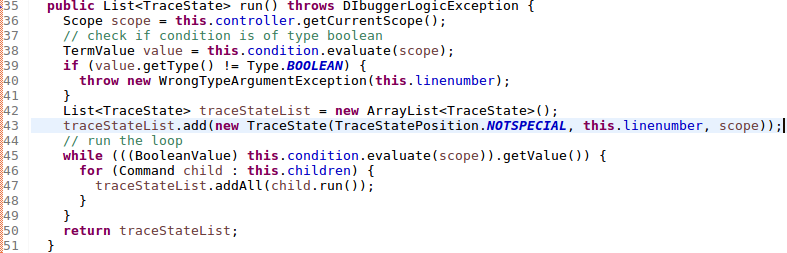
\includegraphics[width=1.0\textwidth]{document_data/runWhile.png}
\caption{run()-Methode der Klasse \textit{WhileCommand}}
\label{runWhile}
\end{figure}
\section{Änderungen zum Entwurf}

\subsection{UserInterface}
\paragraph{ExpressionChangePopUp}
Der Entwurf wurde aus Gründen der Übersichtlichkeit um die Klasse ExpressionChangePopUp, die von DIbuggerPopUp erbt, ergänzt. Ein ExpressionChangePopUp dient dabei dem Löschen und Ändern der Bereichsbindung einer WatchExpression oder eines bedingten Breakpoints.
\paragraph{ArrayValuePopUp}
Die im Entwurf spezifizierte Klasse ArrayValuePopUp, eine Unterklasse von DIbuggerPopUp, wurde in der Implementierung aus Gründen der Benutzerfreundlichkeit verworfen. Ursprünglich sollte sie das Eintragen der Werte eines Arrays über ein PopUp erleichtern. Mit Hilfe eines Scrollbalkens im Variableninspektor ist es allerdings möglich, Werte für Arrays auf dieselbe Art und Weise wie Werte für andere Datentypen einzugeben.
\paragraph{ProgramPanel}
ProgramPanels werden nun nicht mehr über Integers identifiziert, sondern über Strings (A-Z). So ist innerhalb des Modells gewährleistet, dass auch nach Löschung eines einzelnen ProgramPanels die zu den Programmen gehörigen Variablen in Watch-Expressions und bedingten Breakpoints korrekt angezeigt werden.
\subsection{Control}
\paragraph{ExceptionHandler}
Damit Fehlermeldungen in der richtigen Sprache ausgegeben werden, ist der \textit{ExceptionHandler} nun ein Beobachter (im Beobachter-Entwurfsmuster) und beobachtet \textit{FileHandlerInteractor}, um über Änderungen der Benutzersprache informiert zu werden.
\paragraph{FileHandlerInteractor}
Es besteht nun eine Assoziation zwischen \textit{FileHandlerInteractor} und \textit{DebugLogicFacade}, da so \textit{ControlFacade} weniger Funktionalität besitzt, die \textit{FileHandlerInteractor} zuzuordnen ist.
Weiter ist diese Klasse Subjekt im Beobachter-Entwurfsmuster, sodass Objekte anderer Klassen benachrichtigt werden können, falls \textit{FileHandlerInteractor} beispielsweise andere Konfigurationen verwaltet als zuvor.
\paragraph{TextInputBuffer}
Die Klasse \textit{TextInputBuffer} wurde hinzugefügt, um die Parameter der Eingabewerte, Porgrammtexte und -identifikatoren, welche in \textit{Control} zwischenzuspeichern sind, zu kapseln.
Eine Instanz dieser Klasse ermöglicht es genau ein solches \enquote{Tripel} (Eingabewerte, ...) zu speichern und als \textit{ProgramInput}-Objekt wieder abzurufen.
\subsection{FileHandler}
%+ FileHandlerFacade: savePropertiesFile()
\paragraph{Exceptions Paket}
Das Exceptions-Paket sah eine Oberklasse \textit{FileHandlerException} als Interface vor.
Alle Unterklassen, welche diese Schnittstelle implementieren, sollten von der Klasse \textit{java.lang.Exceptions} erben. Da aber Schnittstellen in Java nicht geworfen werden können, wurde die Schnittstelle \textit{FileHandlerException} zu einer abstrakten Klasse mit Erbschaft von \textit{java.lang.Exception}.
\subsection{DebugLogic}
\subsubsection{Debugger}
%+ DebugLogicFacade: extends Observable statt Subject \\
%* DebugLogicFacade: notifyObservers(Object arg); suggestStepSize void statt String \\
%+ DebugControl: setStepSize(programID, stepSize); reset();
\paragraph{Subject}
Im Entwurf wurde die Klasse \textit{Subject} spezifiziert. Sie ist Kontrollpunkt des Beobachtermusters zwischen GUI und DebugLogic. Da eine äquivalente Klasse aus Java, namentlich \textit{Observable}, existiert, wurde die Klasse \textit{Subject} nicht implementiert.
\textit{Observable} biete die gleichen Methoden an, wie unsere definierte Klasse.
\paragraph{DebugLogicFacade}
Diese Klasse erbt nun von der Java Klasse \textit{Observable} anstatt von \textit{Subject}.
Aus den oben genannten Gründen kann somit auch auf die Implementierung der in \textit{Subject} enthaltenen Methoden verzichtet werden.

\subsubsection{Interpreter}
\paragraph{TraceIterator}
Ursprünglich sollte der \textit{TraceIterator} mit Hilfe einer gesonderten Klasse gleichen Namens umgesetzt werden. In der Implementierung wird er nun mittels eines Java-ListIterators über die \textit{TraceState}-Liste innerhalb der Klasse \textit{Trace} verwirklicht. Dieser bietet dieselben Funktionalitäten, kann also in zwei Richtungen iterieren. Um einen Iterator über den Trace zu erhalten, wird weiterhin die Methode \textit{iterator()} der Klasse \textit{Trace} aufgerufen. Diese Entwurfsänderung stellt somit lediglich eine Vereinfachung dar.
\paragraph{TermValue}
Die Klasse \textit{TermValue}, die ursprünglich als Interface implementiert werden sollte, ist nun eine abstrakte Klasse. So kann die Methode \textit{getType()} einmal an zentraler Stelle für alle Unterklassen definiert werden und Code-Duplikate werden vermieden.
\paragraph{TraceState}
In der Klasse \textit{TraceState} wurde das Attribut String programId ergänzt. Dies ist nötig, damit WatchExpressions - die nur TraceStates und keine Traces kennen - wissen, zu welchem Programm welcher TraceState gehört. Dies hat auch eine Änderung in den Klassen \textit{Trace} und \textit{GenerationController} zu Folge. Die Klasse \textit{Trace} übernimmt die Aufgabe, die eben beschriebene \textit{programId} in alle \textit{TraceStates} eines \textit{Traces} einzutragen, und nimmt dazu in ihrem Konstruktor einen weiteren Parameter entgegen. Da der \textit{Trace} diese Information vom  \textit{GenerationController} bekommt, wird auch in Letzterem der Konstruktor erweitert.

\subsubsection{Antlr}
\paragraph{ActuallyHelpfulException und ActuallyHelpfulErrorListener}
Ursprünglich sollte das gesamte Antlr-Paket autogeneriert werden. Allerdings mussten zur Behandlung von Exceptions zwei Klassen hinzugefügt werden, da Antlr standardmäßig alle Fehlermeldungen auf das Terminal schreibt, statt sie zu werfen.

 

\end{document}
